\begin{figure}[htbp]
\centering
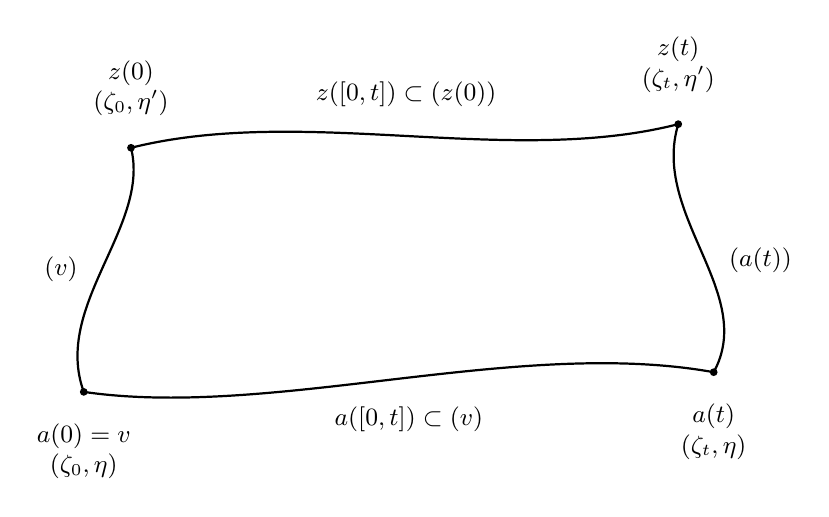
\begin{tikzpicture}[x=1cm,y=1cm,font=\small]
  \coordinate (v) at (0,0);
  \coordinate (a) at (8,0.25);
  \coordinate (z0) at (0.6,3.1);
  \coordinate (zt) at (7.55,3.4);
  \draw[thick] (v) .. controls (2.4,-0.35) and (5.5,0.7) .. (a)
    node[pos=0.52,below=7pt] {$a([0,t])\subset\Ws(v)$};
  \draw[thick] (z0) .. controls (2.8,3.65) and (5.4,2.85) .. (zt)
    node[pos=0.50,above=7pt] {$z([0,t])\subset\Ws(z(0))$};
  \draw[thick] (v) .. controls (-0.4,1.1) and (0.85,2.1) .. (z0)
    node[pos=0.49,left=5pt] {$\Wu(v)$};
  \draw[thick] (a) .. controls (8.55,1.25) and (7.2,2.25) .. (zt)
    node[pos=0.47,right=5pt] {$\Wu(a(t))$};
  \fill (v) circle (1.4pt);
  \fill (a) circle (1.4pt);
  \fill (z0) circle (1.4pt);
  \fill (zt) circle (1.4pt);
  \node[below=8pt,align=center] at (v)
    {$a(0)=v$\\$ (\zeta_0,\eta)$};
  \node[below=8pt,align=center] at (a)
    {$a(t)$\\$ (\zeta_t,\eta)$};
  \node[above=8pt,align=center] at (z0)
    {$z(0)$\\$ (\zeta_0,\eta')$};
  \node[above=8pt,align=center] at (zt)
    {$z(t)$\\$ (\zeta_t,\eta')$};
\end{tikzpicture}
\caption{Actual leaf incidences in the infinite-dimensional alternative,
for a fixed finite $t$. Each ordered pair gives the past and future
endpoints. The lower path is tangent to $P^s$; the translated upper
path is proved tangent to $E^s$. Each vertical connection indicates
membership in one strong unstable leaf. The drawing is schematic:
it asserts no ambient affine plane, smooth product chart or embedded
surface. The contradiction uses the proper lower ray and the endpoint
identities, not any geometric shape of this drawing.}
\label{fig:mixed-rectangle}
\end{figure}
